\documentclass[conference]{IEEEtran}
\usepackage{cite}
\usepackage{amsmath}
\usepackage{newtxtext,newtxmath}
\usepackage{graphicx}
\usepackage{url}

\begin{document}

\title{Hybrid Classical--Neural Detection of Voice Pathology from Sustained Vowels with Cross-Database Evaluation}

\author{\IEEEauthorblockN{Mustafa Mert S\"uerkan}
\IEEEauthorblockA{\textit{Computer Engineering Department} \\
\textit{TED University}\\
Ankara, Turkey \\
Email: mmert.suerkan@tedu.edu.tr}}

\maketitle

\begin{abstract}
We propose a non-invasive screening system that labels a short sustained-vowel recording as \emph{healthy} or \emph{pathological}. The system combines hand-implemented classical speech analysis---the short-time Fourier transform (STFT), mel-frequency cepstral coefficients (MFCC), linear predictive coding (LPC), and pitch-perturbation measures---with a lightweight convolutional neural network (CNN) in a late-fusion architecture. An MFCC--Gaussian mixture model (GMM) classifier serves as the baseline. The system is trained on the public Saarbr\"ucken Voice Database (SVD) under a speaker-independent protocol and tested, without retraining, on the independent VOICED database recorded with different equipment.
\end{abstract}

\begin{IEEEkeywords}
voice pathology detection, MFCC, linear prediction, jitter and shimmer, CNN, cross-database evaluation
\end{IEEEkeywords}

\section{Problem and Motivation}
Pathologies such as nodules, polyps, laryngitis, and vocal-fold paralysis change how the vocal folds vibrate. The result is a voice that sounds hoarse, breathy, or rough. A clinical examination is the reference standard, but it requires an otolaryngologist and dedicated equipment. A recording-based screening tool could flag at-risk speakers early and support remote follow-up. It is a decision-support aid, not a replacement for diagnosis.

Many studies report high accuracy on the SVD. However, Huckvale and Buciuleac~\cite{huckvale2021} showed that these numbers are hard to compare: papers use different pathology subsets, audio materials, and cross-validation schemes. When three published systems were re-implemented under one protocol, the differences between them largely disappeared. End-to-end deep learning on small clinical data is not automatically better either: a convolutional--recurrent network trained on raw SVD vowels reached 68\% accuracy~\cite{harar2017}.

In the source--filter model of speech production~\cite{rabiner2007}, voice pathologies act mainly on the \emph{source} (vocal-fold vibration). Spectral-envelope features such as MFCCs~\cite{davis1980} mostly describe the \emph{filter} (the vocal tract). We therefore combine envelope features, source-related measures (LPC residual, F0 perturbation), and a learned spectro-temporal representation, and evaluate them under a strict protocol.

\section{Research Questions}
\textbf{RQ1:} Under a speaker-independent protocol, does late fusion of a CNN on log-mel spectrograms with interpretable MFCC/LPC/perturbation features outperform an MFCC--GMM baseline?
\textbf{RQ2:} Which feature family---envelope (MFCC), source (LPC residual, jitter, shimmer), or learned (CNN)---transfers best to a database recorded with different equipment and at a different sampling rate?
\textbf{RQ3:} Is performance consistent across sexes, or does the classifier rely on sex-related cues?

\section{Data}
\textbf{SVD}~\cite{svd,puetzer2008}: German speakers recorded at 50\,kHz, 16-bit. It contains 1002 speakers with a wide range of voice disorders and 851 controls~\cite{huckvale2021}. Each session has /a/, /i/, /u/ at normal, high, low, and rising--falling pitch, plus one sentence. The database is released on Zenodo under CC~BY~4.0 (DOI 10.5281/zenodo.16874898). Of the 38\,GB release, only the normal-pitch /a/ recordings are used, converted from \texttt{.nsp} to \texttt{.wav} with the published converter.

\textbf{VOICED}~\cite{voiced2018}: 208 recordings of a 5\,s sustained /a/, sampled at 8\,kHz and released on PhysioNet under the ODC Attribution License. It is used \emph{only} as an external test set.

\begin{table}[h]
\caption{Databases (SVD: speakers in the full database~\cite{huckvale2021}).}
\label{tab:data}
\centering
\begin{tabular}{lccc}
\hline
Database & Healthy / Path. & Fs & Role \\
\hline
SVD & 851 / 1002 spk. & 50\,kHz & train / CV \\
VOICED & 58 / 150 rec. & 8\,kHz & external test \\
\hline
\end{tabular}
\end{table}

\textbf{Task:} binary classification, healthy vs.\ any pathology. Sessions from the same speaker are always kept in the same fold to prevent speaker leakage (some SVD speakers have many sessions~\cite{huckvale2021}). For the cross-database experiment, the SVD is downsampled to 8\,kHz with an anti-aliasing filter so that the training and test bandwidths match.

\section{Methodology}
\textbf{Front end (implemented from scratch in NumPy, CS\,568 topics):}
\begin{itemize}
\item \emph{STFT and MFCC} (L6, L9): pre-emphasis, 25\,ms Hamming-windowed frames with a 10\,ms hop, and an FFT, followed by a 40-band mel filterbank, logarithm, and DCT-II. This gives 13 MFCCs plus $\Delta$ coefficients; the same filterbank output without the DCT is the log-mel spectrogram used by the CNN.
\item \emph{LPC} (L7): order-16 LPC with the autocorrelation method and the Levinson--Durbin recursion~\cite{makhoul1975}. From it, the first three formants and their bandwidths (polynomial roots) are derived. Inverse filtering gives the prediction residual $e[n]=s[n]-\sum_{k=1}^{p}a_k\,s[n-k]$, an estimate of the excitation. Its normalized energy and kurtosis are computed.
\item \emph{Source/perturbation} (L8): F0 is estimated by autocorrelation. Local jitter and shimmer are computed from consecutive period lengths $T_i$ and peak amplitudes $A_i$; for example, $\text{jitter}=\frac{1}{N-1}\sum_i|T_i-T_{i+1}|\,/\,\bar{T}$.
\end{itemize}
Frame-level features are summarized per recording (mean, standard deviation); every block is unit-tested against a reference library.

\begin{figure}[t]
\centering
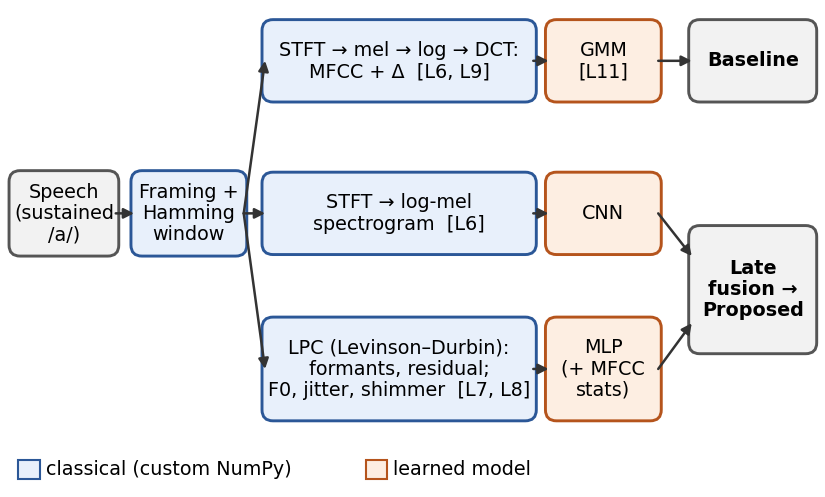
\includegraphics[width=\columnwidth]{fig_pipeline.png}
\caption{Pipeline. Blue: classical analysis implemented from scratch (lecture numbers in brackets). Orange: learned models.}
\label{fig:pipeline}
\end{figure}

\textbf{Hypothesis:} pathologies disturb the regularity of the glottal source more than the vocal-tract envelope. Source descriptors should therefore add information that MFCCs and spectrograms do not capture, especially when the recording channel changes.

\textbf{Baseline:} two diagonal-covariance GMMs~\cite{reynolds1995} (healthy, pathological) trained on frame-level MFCC+$\Delta$ vectors. A recording is classified by the log-likelihood ratio summed over its frames, and the number of mixtures is chosen by inner cross-validation.

\textbf{Proposed (Fig.~\ref{fig:pipeline}):}
\begin{itemize}
\item a small CNN (three convolutional blocks with batch normalization and pooling, then global average pooling) on a fixed-length log-mel excerpt;
\item a two-layer MLP on the standardized vector of MFCC statistics, LPC features, and perturbation measures;
\item concatenation of the two embeddings followed by a sigmoid output (late fusion).
\end{itemize}
Training uses class-weighted binary cross-entropy and early stopping. \textbf{Ablations:} CNN only, envelope features only, source features only, and full fusion.

\section{Evaluation Protocols}
\textbf{P1:} speaker-independent, stratified 5-fold cross-validation on the SVD, following the common protocol of~\cite{huckvale2021}. \textbf{P2:} cross-database transfer---train on the full SVD at 8\,kHz, test on VOICED without fine-tuning (RQ2). \textbf{P3:} results broken down by sex, plus a sex-balanced re-sampled training run (RQ3). \textbf{P4:} the ablations above, evaluated under both P1 and P2. \textbf{Metrics:} unweighted average recall (UAR, the primary metric because the classes are imbalanced), F1, sensitivity, specificity, and ROC AUC, reported as mean $\pm$ standard deviation over folds. Systems are compared with paired tests over folds.

\textbf{Compute and reproducibility:} Google Colab with data, cached \texttt{.npy} features, and checkpoints on Google Drive. Code, fold definitions, and configurations will be public on GitHub (\url{https://github.com/mmsuerkan/voice-pathology-detection}).

\textbf{Risks and mitigations:} (i)~small, imbalanced data---a compact CNN, class weighting, and early stopping; (ii)~pitch tracking may fail on severely pathological voices---frames where tracking fails are masked, and their proportion is itself used as a feature; (iii)~the sampling-rate mismatch between the databases---resolved by training at 8\,kHz for P2.

\textbf{Timeline:} by 20 Nov, data and front end with unit tests; by 4 Dec, GMM baseline and the cross-validation framework; by 18 Dec, CNN, fusion, ablations, and P2--P3; by 25 Dec, final paper and code; 28 Dec--1 Jan, presentation.

\textbf{Expected outcomes:} a reproducible, speaker-independent comparison of classical, learned, and fused features; an estimate of how much accuracy survives a change of database; and evidence on whether source descriptors add information beyond envelope and CNN features.

\begin{thebibliography}{9}
\bibitem{huckvale2021}
M.~Huckvale and C.~Buciuleac, ``Automated detection of voice disorder in the Saarbr\"ucken voice database: Effects of pathology subset and audio materials,'' in \emph{Proc. Interspeech}, 2021, pp.~1399--1403.

\bibitem{harar2017}
P.~Harar, J.~B.~Alonso-Hern\'andez, J.~Mekyska, Z.~Gal\'a\v{z}, R.~Burget, and Z.~Sm\'ekal, ``Voice pathology detection using deep learning: A preliminary study,'' in \emph{Proc. IWOBI}, 2017, pp.~45--48.

\bibitem{rabiner2007}
L.~R.~Rabiner and R.~W.~Schafer, ``Introduction to digital speech processing,'' \emph{Found. Trends Signal Process.}, vol.~1, no.~1--2, pp.~1--194, 2007.

\bibitem{davis1980}
S.~B.~Davis and P.~Mermelstein, ``Comparison of parametric representations for monosyllabic word recognition in continuously spoken sentences,'' \emph{IEEE Trans. Acoust., Speech, Signal Process.}, vol.~28, no.~4, pp.~357--366, 1980.

\bibitem{svd}
M.~P\"utzer and W.~J.~Barry, \emph{Saarbr\"ucken Voice Database} (v2), Zenodo, 2008, doi: 10.5281/zenodo.16874898.

\bibitem{puetzer2008}
M.~P\"utzer and W.~J.~Barry, ``Instrumental dimensioning of normal and pathological phonation using acoustic measurements,'' \emph{Clin. Linguist. Phon.}, vol.~22, no.~6, pp.~407--420, 2008.

\bibitem{voiced2018}
U.~Cesari, G.~De~Pietro, E.~Marciano, C.~Niri, G.~Sannino, and L.~Verde, ``A new database of healthy and pathological voices,'' \emph{Comput. Electr. Eng.}, vol.~68, pp.~310--321, 2018.

\bibitem{makhoul1975}
J.~Makhoul, ``Linear prediction: A tutorial review,'' \emph{Proc. IEEE}, vol.~63, no.~4, pp.~561--580, 1975.

\bibitem{reynolds1995}
D.~A.~Reynolds and R.~C.~Rose, ``Robust text-independent speaker identification using Gaussian mixture speaker models,'' \emph{IEEE Trans. Speech Audio Process.}, vol.~3, no.~1, pp.~72--83, 1995.
\end{thebibliography}

\end{document}
